\subsubsection{Administrator application -- Java Swing}
\label{subsubsec:client-admin}

The V1 administrator interface is built with Java Swing on Windows, for managing
and monitoring the system. The list below assigns the function codes used to map
functions to the tasks in Section~\ref{subsec:task-plan}.
The subsystem of the functions in this table is the system Admin, which is not the
same as the group admin role in a chat group.

\begingroup
\small
\begin{longtable}{|C{1.2cm}|L{\dimexpr\textwidth-1.2cm-4\tabcolsep-3\arrayrulewidth\relax}|}
  \caption{Functions of the administrator subsystem}
  \label{tab:admin-features}\\
  \hline
  \textbf{Code} & \textbf{Function and scope}\\
  \hline
  \endfirsthead
  \hline
  \textbf{Code} & \textbf{Function and scope}\\
  \hline
  \endhead
  \hypertarget{F13}{\texttt{F13}} &
  \textbf{Manage accounts:} view, add, update, delete; lock/unlock accounts;
  update passwords; view a user's sign-in history and friend list.
  User information includes the username, full name, address, date of birth,
  gender and email.
  Filter by name, username or status; sort by name or creation date.\\
  \hline
  \hypertarget{F14}{\texttt{F14}} &
  \textbf{View sign-ins:} show the time, username and full name,
  in time order.\\
  \hline
  \hypertarget{F15}{\texttt{F15}} &
  \textbf{View chat groups:} filter by name; sort by name or creation time;
  view the members and admins of each group.\\
  \hline
  \hypertarget{F16}{\texttt{F16}} &
  \textbf{View and handle spam reports:} filter by year and username;
  sort by time or username; lock the reported account.\\
  \hline
  \hypertarget{F17}{\texttt{F17}} &
  \textbf{View new registrations:} choose a year, filter by name,
  sort by name or creation time.\\
  \hline
  \hypertarget{F18}{\texttt{F18}} &
  \textbf{Registrations chart:} choose a year and show the number of new
  registrations per month; the horizontal axis is the month, the vertical axis
  the number of new registrations.\\
  \hline
  \hypertarget{F19}{\texttt{F19}} &
  \textbf{Friend statistics:} show the number of direct friends and the count
  including friends of friends; filter by name and by the number of direct friends
  equal to, less than or greater than an entered value; sort by name or creation time.\\
  \hline
  \hypertarget{F20}{\texttt{F20}} &
  \textbf{View active users:} choose a year; see the number of app opens and how
  many people and groups were chatted with; filter by name and by activity count
  equal to, less than or greater than an entered value;
  sort by name or creation time.\\
  \hline
  \hypertarget{F21}{\texttt{F21}} &
  \textbf{Active users chart:} choose a year and show the number of people who
  opened the app each month; the horizontal axis is the month, the vertical axis
  the number of people who opened the app.\\
  \hline
\end{longtable}
\endgroup

In V1, this list is used to check the administrator screens against the
requirements, including the matching action, filter and sort controls.

\paragraph{Navigation and screen list}
\label{par:admin-navigation}
\mbox{}\par
The left sidebar is split into \textbf{Manage Accounts},
\textbf{Monitor \& Moderate} and \textbf{Analyze Usage}. When the V1 preview starts,
the application opens the \textbf{Admin Sign in} screen; after signing in, the
\textbf{Users} screen is shown. Table~\ref{tab:admin-screen-map}
maps the Swing interface to the Figma prototype~\cite{ref:figma} and to the
function codes of the assignment. Labels in the table are quoted from the interface.

\begingroup
\small
\begin{longtable}{|L{4.3cm}|L{\dimexpr\textwidth-4.3cm-4\tabcolsep-3\arrayrulewidth\relax}|}
  \caption{V1 administrator screens}
  \label{tab:admin-screen-map}\\
  \hline
  \textbf{Screen} & \textbf{Functions and content}\\
  \hline
  \endfirsthead
  \hline
  \textbf{Screen} & \textbf{Functions and content}\\
  \hline
  \endhead
  Admin Sign in
  & The administrator application's own sign-in screen, separate from the sign-in
  screen of the user application. It has a username, a password and a message when
  a field is empty. In V2 the server checks the password and the \texttt{ADMIN} role
  before opening a session; \textbf{Sign Out} returns to this screen.\\
  \hline
  \href{https://www.figma.com/design/maCogjZs9eOOhfkxsOZoIU?node-id=2-80}{Users}
  & \hyperlink{F13}{F13}. Account list and profile, add/edit form,
  password change, lock/unlock and delete confirmation. The profile has the
  \textbf{Login History} and \textbf{Friends \& Groups} tabs. The address and date of
  birth are optional. The account status is \textbf{Active} or \textbf{Locked};
  a locked account stays locked until an administrator unlocks it.\\
  \hline
  \href{https://www.figma.com/design/maCogjZs9eOOhfkxsOZoIU?node-id=16-822}{Account History}
  & \hyperlink{F14}{F14}, \hyperlink{F17}{F17}. \textbf{Sign-ins} shows the time,
  username and full name across the whole system. \textbf{New Accounts}
  shows the accounts created in the selected year, with search, sorting and a monthly
  registrations chart.\\
  \hline
  \href{https://www.figma.com/design/maCogjZs9eOOhfkxsOZoIU?node-id=25-1020}{Chat Groups}
  & \hyperlink{F15}{F15}. Group list with search and sorting. The group detail
  shows the creator, the creation time, the members and the group admins.
  \textbf{Activity} and \textbf{Monitoring} illustrate an extension for monitoring
  groups. The monthly chart counts activity, messages or members joining.\\
  \hline
  \href{https://www.figma.com/design/maCogjZs9eOOhfkxsOZoIU?node-id=38-1461}{Spam Reports}
  & \hyperlink{F16}{F16}. \textbf{Reports} lists the individual reports.
  \textbf{By account} groups them by account, with a status filter and the report
  history. The lock count and the lock/unlock log use the same selected year.
  The report detail shows the reporter, the reported account, the reason and the
  related message before the account lock is confirmed.\\
  \hline
  \href{https://www.figma.com/design/maCogjZs9eOOhfkxsOZoIU?node-id=53-934}{Analytics / Overview}
  & \hyperlink{F18}{F18}, \hyperlink{F21}{F21}. \textbf{Graph} selects the monthly
  chart for the year. \textbf{Registrations} counts created accounts;
  \textbf{Active users} counts distinct accounts that opened the app. The
  \textbf{Sign-ins} and \textbf{Messages sent} charts add more views of usage.\\
  \hline
  \href{https://www.figma.com/design/maCogjZs9eOOhfkxsOZoIU?node-id=53-1087}{Analytics / Friend Counts}
  & \hyperlink{F19}{F19}. The table shows the number of direct friends and the total
  number of people in the friend network. An account's detail has three collapsible
  lists: friends, chat groups, and friends of friends with their mutual friends.\\
  \hline
  \href{https://www.figma.com/design/maCogjZs9eOOhfkxsOZoIU?node-id=53-1279}{Analytics / Activity}
  & \hyperlink{F20}{F20}. The table for the selected year shows sign-ins, app opens,
  and the number of people and groups chatted with, each separately. By default
  \textbf{Any count} also shows accounts that opened the app without signing in
  again in the selected year. The \textbf{Monthly sign-ins} chart counts system-wide
  sign-ins in each month of that year. The \textbf{Active users} chart on
  \textbf{Overview} counts distinct accounts that opened the app.\\
  \hline
\end{longtable}
\endgroup

\paragraph{Period picker}
\mbox{}\par
The team applies the ``time period'' of the assignment (new registrations, active
users and filtering spam reports by time) as a calendar year, in line with the
yearly charts.
The \textbf{Period} button selects one calendar year shared by every administrator
screen that has a time filter. The selected year is kept when switching screens.
Time-based lists show the records from 1 January to 31 December of that year.
Every chart shows all 12 months from January to December, even when some months or
the whole year have no records.

\paragraph{V1 Java Swing screenshots}
\mbox{}\par
The screenshots below are rendered from the Java Swing application in the
\texttt{admin-client} module. The V1 build opens the \textbf{Admin Sign in} screen,
then the \textbf{Users} screen, and uses in-memory sample data. In V1 the sign-in
screen accepts any non-empty username and password (for example
\texttt{admin} / \texttt{admin}); the server checks the \texttt{ADMIN} role in V2. The
sample data is the same as in the user application. The administrator's display
name is \textbf{Admin}. Account changes last only for the preview session. The
password change form shows the input checks.

\noindent\begin{minipage}{\linewidth}
  \centering
  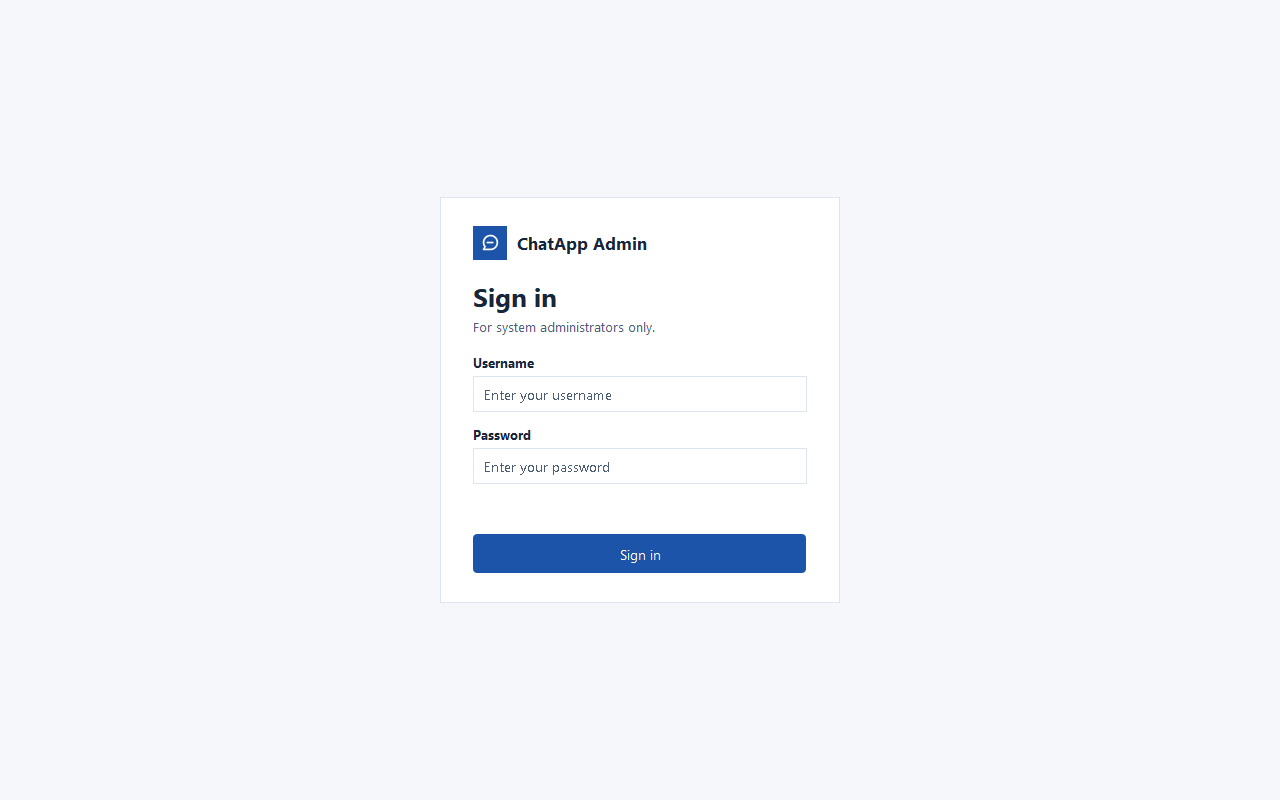
\includegraphics[width=.74\linewidth]{images/admin-swing-login.png}
  \captionof{figure}{Sign-in screen of the administrator application.}
  \label{fig:admin-swing-login}
\end{minipage}

\noindent\begin{minipage}{\linewidth}
  \centering
  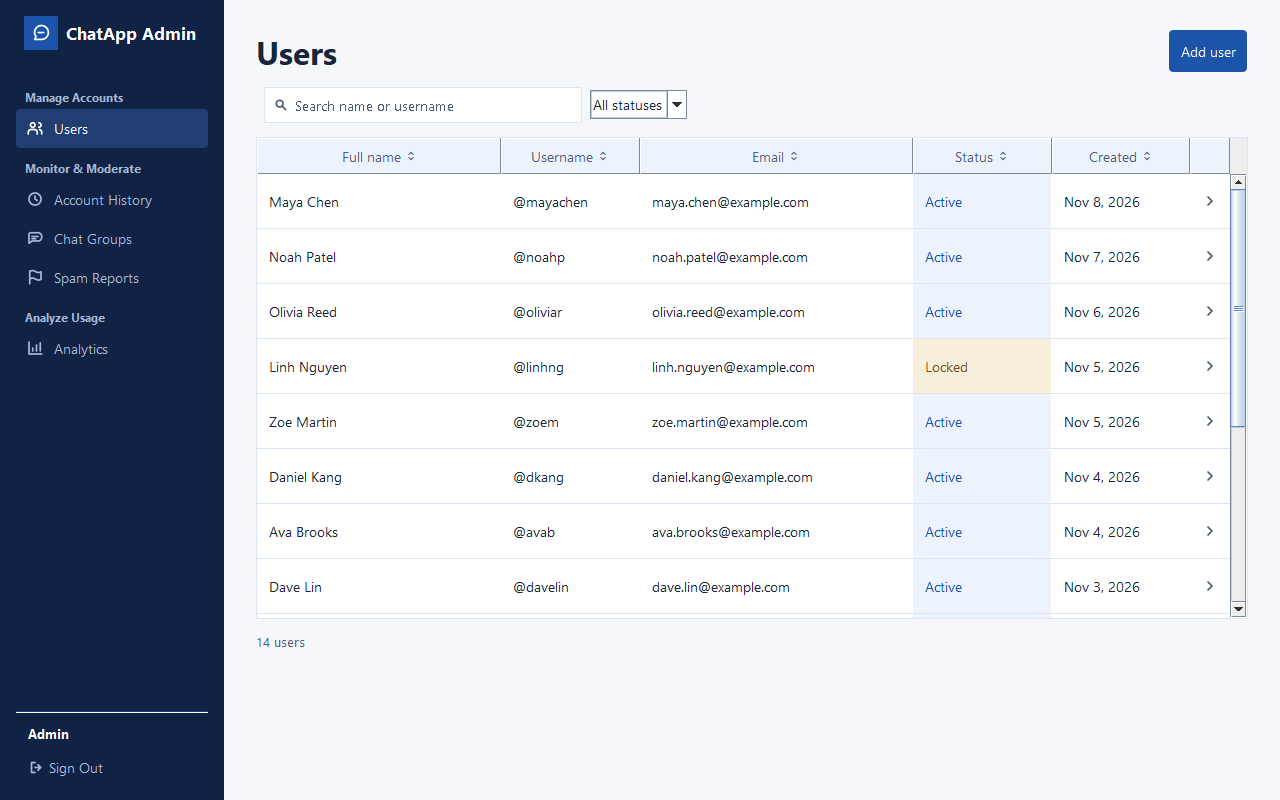
\includegraphics[width=.48\linewidth]{images/admin-swing-users.png}\hfill
  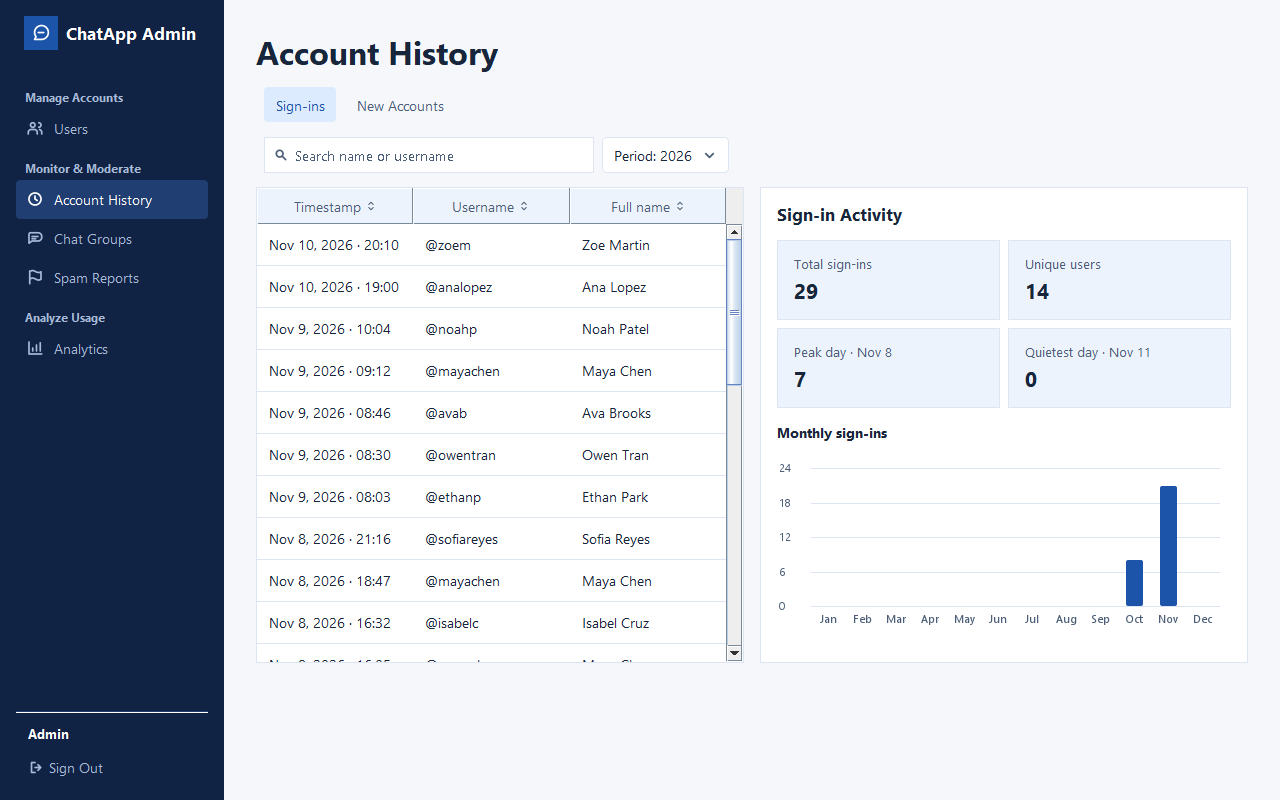
\includegraphics[width=.48\linewidth]{images/admin-swing-account-history.png}
  \captionof{figure}{F13 and F14. Account list and system-wide sign-in history.}
  \label{fig:admin-swing-users-history}
\end{minipage}

\noindent\begin{minipage}{\linewidth}
  \centering
  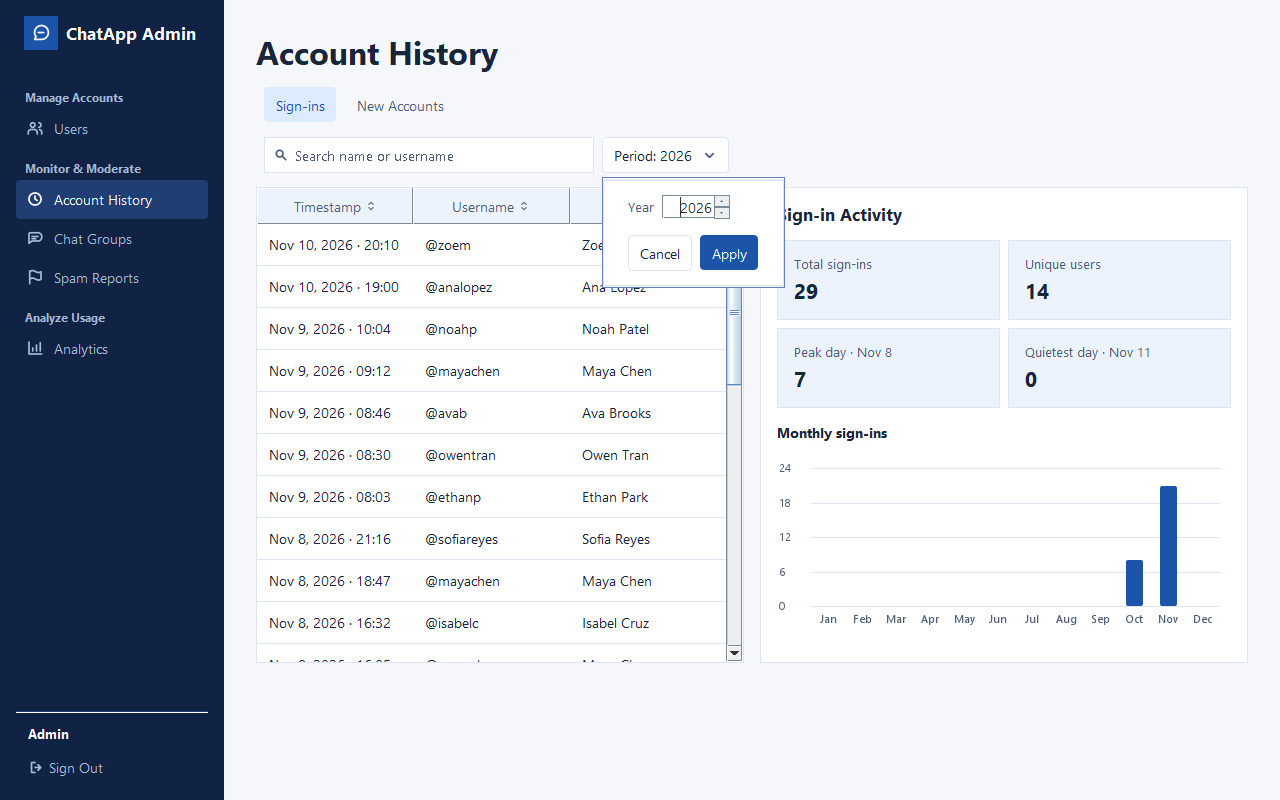
\includegraphics[width=.92\linewidth]{images/admin-swing-period-picker.png}
  \captionof{figure}{The shared year picker, opened from the Account History screen.}
  \label{fig:admin-swing-period}
\end{minipage}

\noindent\begin{minipage}{\linewidth}
  \centering
  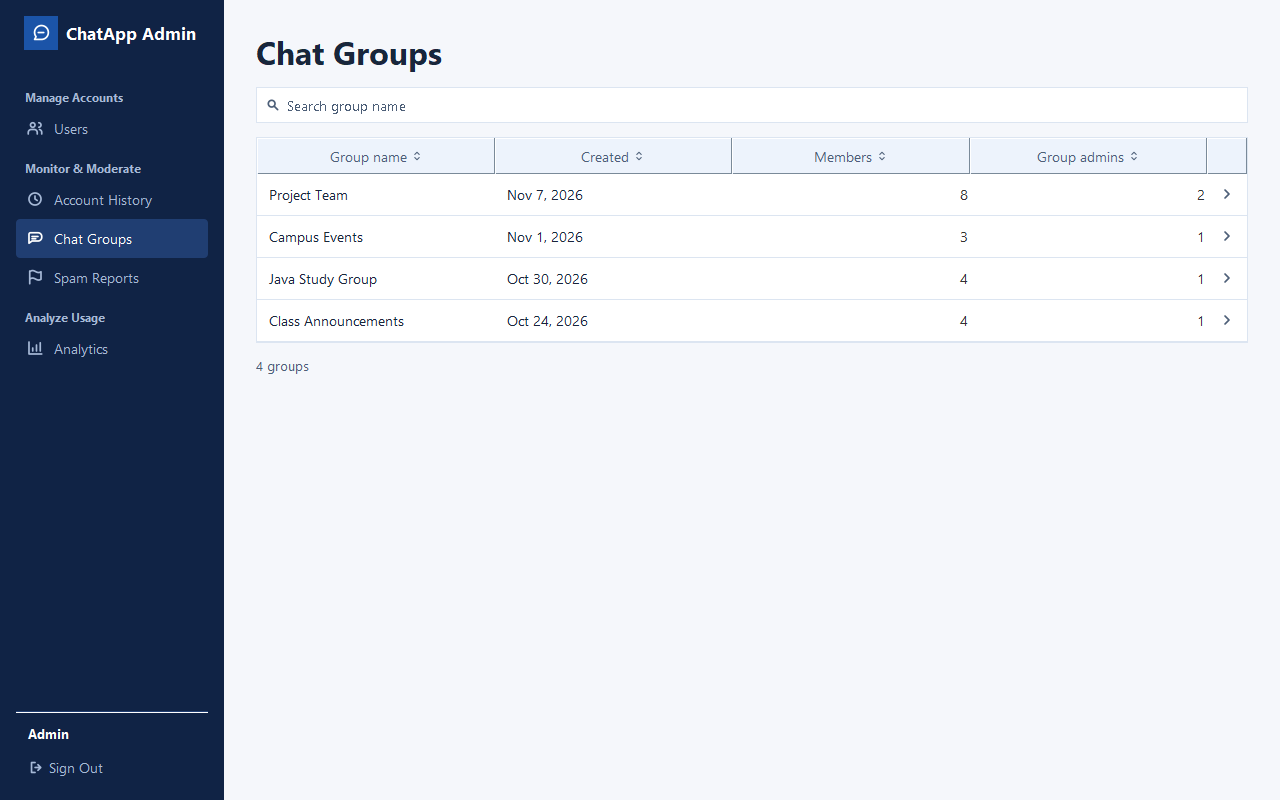
\includegraphics[width=.48\linewidth]{images/admin-swing-groups.png}\hfill
  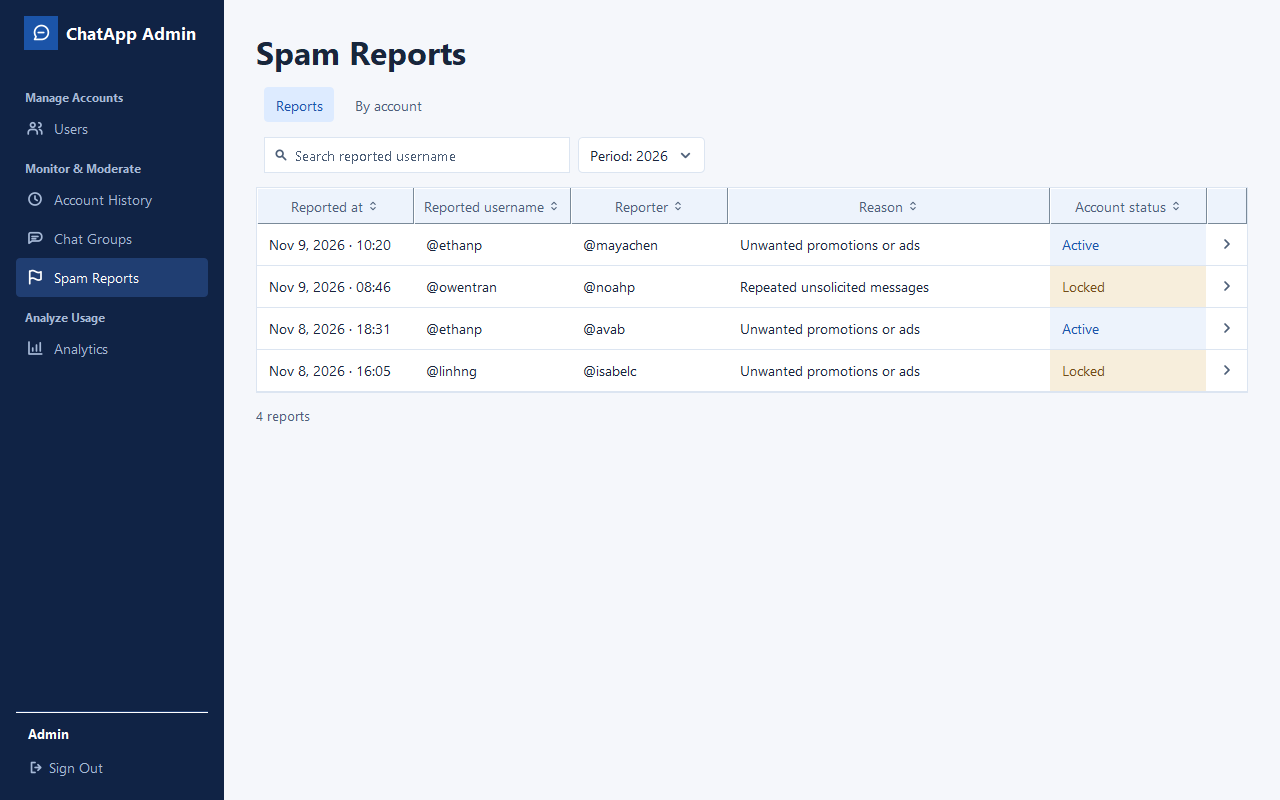
\includegraphics[width=.48\linewidth]{images/admin-swing-spam-reports.png}
  \captionof{figure}{F15 and F16. Chat groups and spam reports.}
  \label{fig:admin-swing-moderation}
\end{minipage}

\noindent\begin{minipage}{\linewidth}
  \centering
  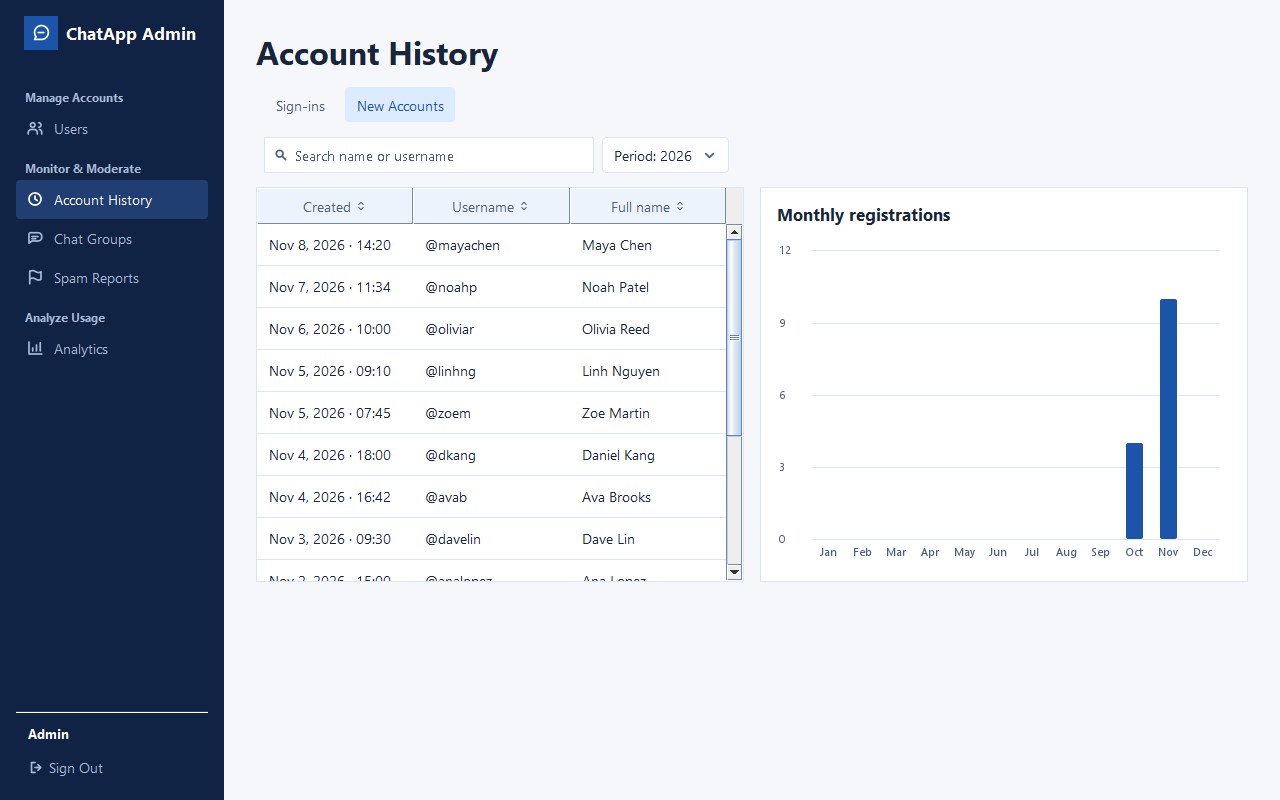
\includegraphics[width=.48\linewidth]{images/admin-swing-new-accounts.png}\hfill
  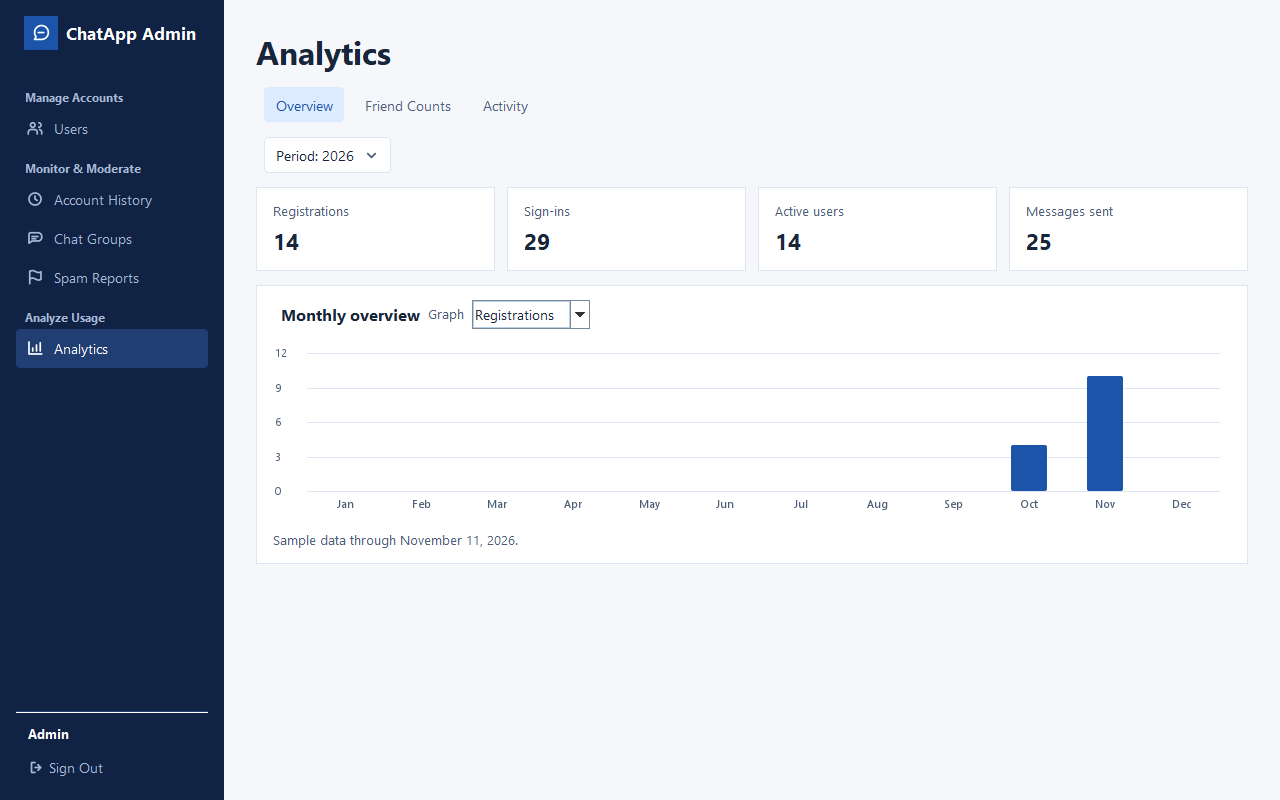
\includegraphics[width=.48\linewidth]{images/admin-swing-overview.png}
  \captionof{figure}{F17 and F18. New accounts in the selected year and the monthly registrations chart.}
  \label{fig:admin-swing-registrations}
\end{minipage}

\noindent\begin{minipage}{\linewidth}
  \centering
  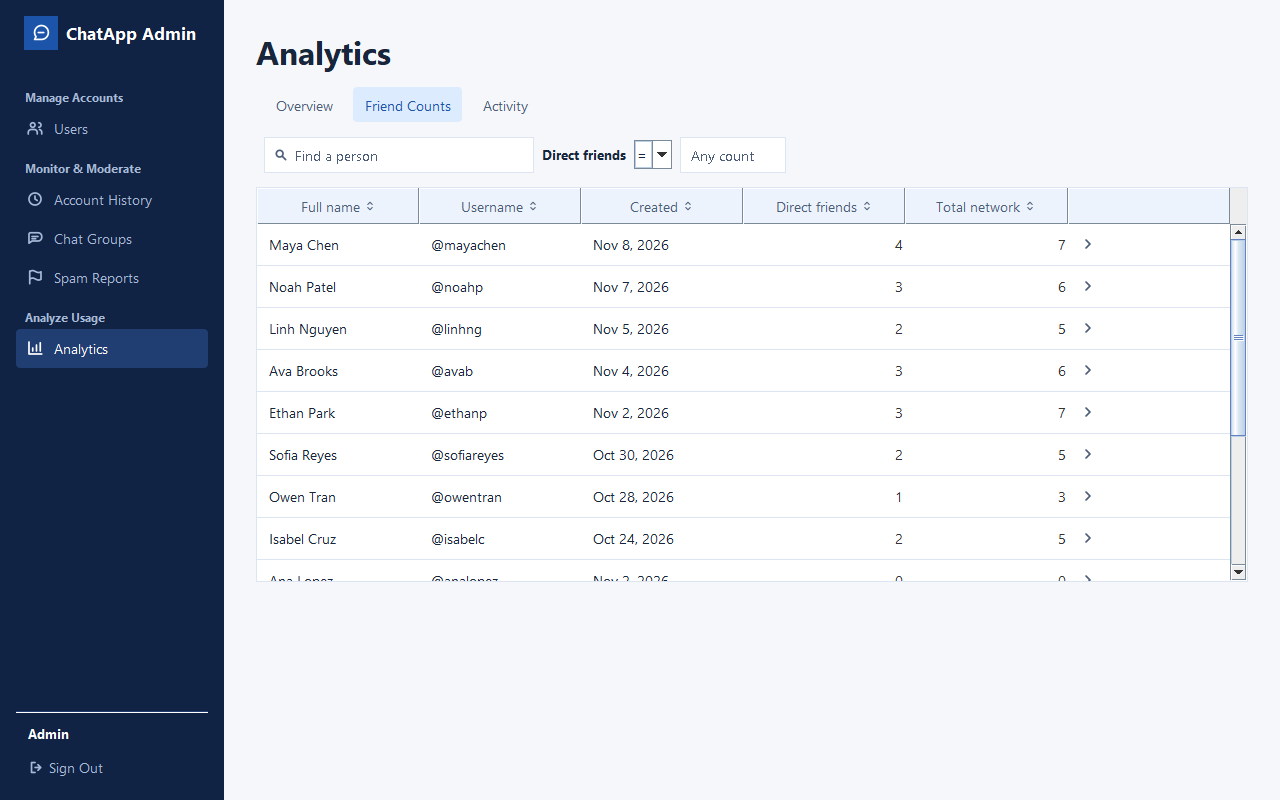
\includegraphics[width=.48\linewidth]{images/admin-swing-friend-counts.png}\hfill
  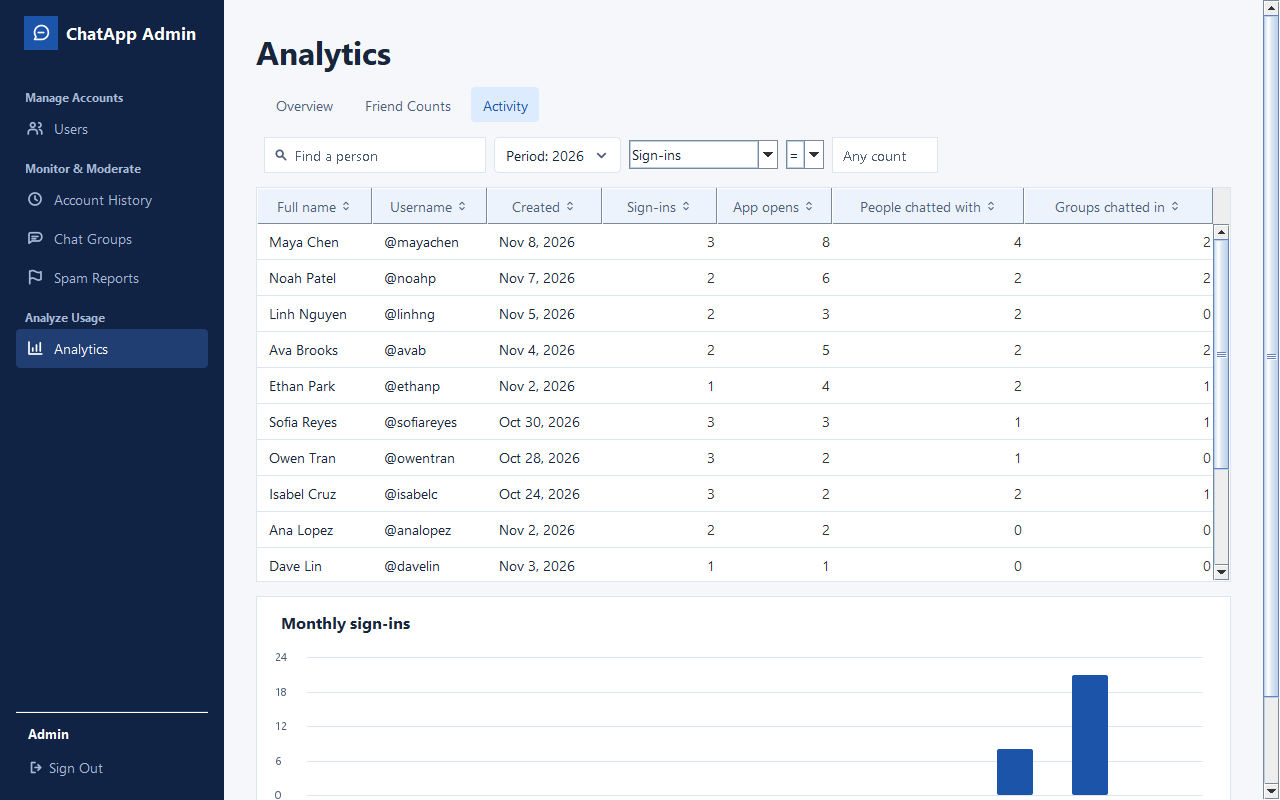
\includegraphics[width=.48\linewidth]{images/admin-swing-activity.png}
  \captionof{figure}{F19 and F20. Friend statistics and activity per account.}
  \label{fig:admin-swing-friends-activity}
\end{minipage}

\noindent\begin{minipage}{\linewidth}
  \centering
  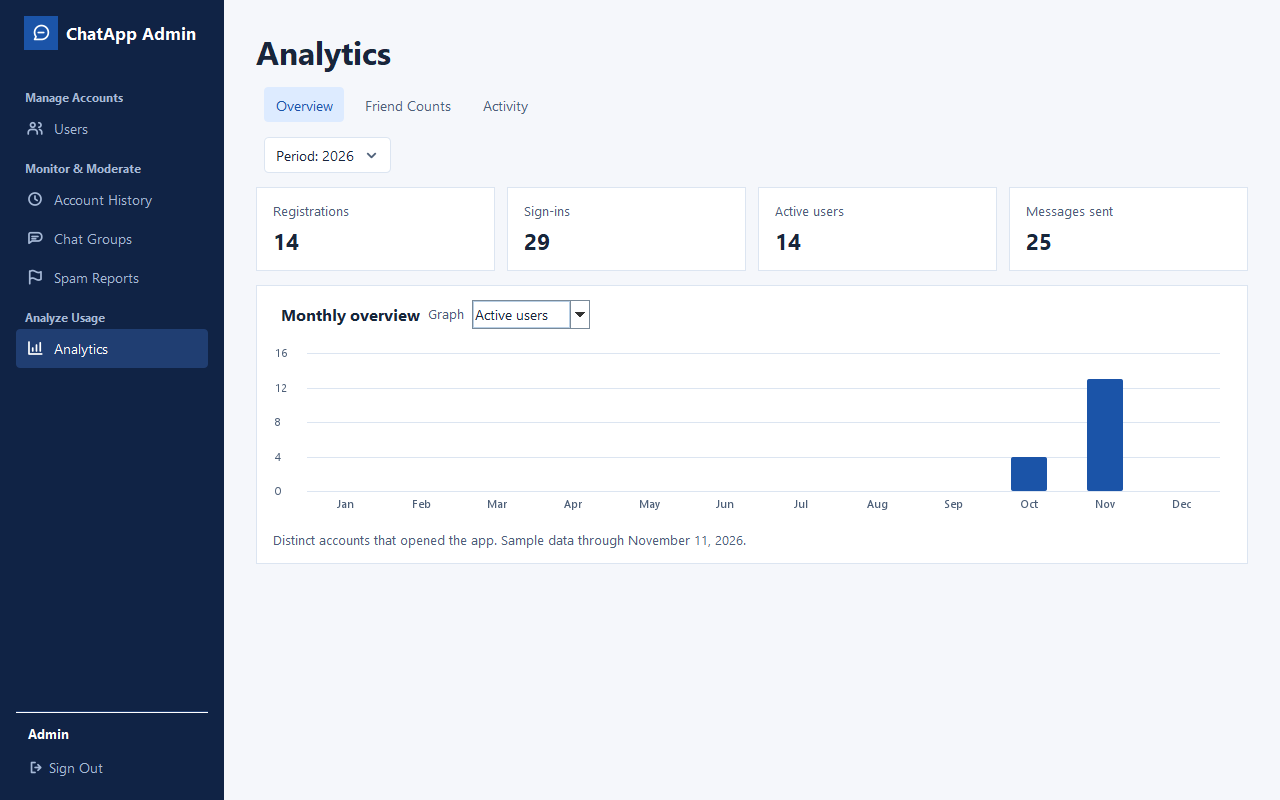
\includegraphics[width=.74\linewidth]{images/admin-swing-active-users.png}
  \captionof{figure}{F21. Distinct accounts that opened the app in each month.}
  \label{fig:admin-swing-active-users}
\end{minipage}
